\documentclass[11pt,a4paper,oneside]{article}
\usepackage[latin1]{inputenc}
\usepackage{amsmath}
\usepackage{amsfonts}
\usepackage{amssymb}
\usepackage{graphicx}
\usepackage{color}
\usepackage {tikz}
\usepackage{fancyvrb}
\usetikzlibrary {er}
\usepackage[left=2.00cm, right=2.00cm, top=1.00cm]{geometry}
\graphicspath{{./}}
\fvset{tabsize=4}

\begin{document}
	\title{DS 255 - System Virtualization \\ Assignment IV - System Virtual Machines}
	\author{Shriram R. \\ M Tech (CDS) \\ 06-02-01-10-51-18-1-15763}
	\maketitle	
	
	\begin{enumerate}
		\item It is important for VMM to handle the timer interrupt as it provides an opportunity for gaining control of the system to enable the time sharing of resources among different guest VMs. When a timer interrupt occurs, the VMM executes a code which performs the following operations
		\begin{enumerate}
			\item Save the architected state of running VM and determine the next VM to be activated
			\item Restore the architected state for next VM and set timer interval and enable interrupts
			\item Set PC to timer interrupt handler of OS in next VM
		\end{enumerate}
	    The guest OS must be denied direct access to timer interrupt to ensure a fair scheme of time sharing of resources to work. Otherwise, the guest will have access to reschedule the next timer interrupt which can degrade performance of other running VMs. This is why the guest OS is provided with virtual emulated timer interrupt by the VMM.
	    
	    Also, it might not be feasible to ensure transparency by VMM if the guest is allowed to read the real timer interrupt value set by the VMM. Lack of transparency might cause the guest OS to behave differently when running under a VMM than a real machine.
		
		\item The consequences of running multiple OSes without hypervisors are as follows,
		\begin{enumerate}
			\item The performance isolation and security should now be enforced by hardware in general
            \item Different ISA emulation is now a challenge due to the absence of hypervisor
            \item VM creation including resource allocation \& mgmt. has to be performed by the hardware
		\end{enumerate}
	    This type of configuration requires hardware or the ISA to provide hypervisor capabilities including VM management, isolation, emulation etc. This means that the hardware emulates the privileged role of a hypervisor leading to hardware based virtualization.
		
		\item There are different variants for the standard time-sharing CPU scheduler as implemented in \emph{Xen} hypervisor. They are: (a) Borrowed Virtual Time (BVT) scheduler, (b) Simple Earliest Deadline First (SEDF) scheduler and (c) Credit Scheduler. 
		
		For the given scenario of three VMs on top of a single CPU, SEDF scheduler can be used. The goals of this scheduler is to increase \emph{fairness} which is the time interval over which the scheduler provides fair CPU allocation and decrease \emph{allocation error} which is the relative difference between requested CPU use percentage and the actual/observed CPU use percentage for a given VM.
		
		The SEDF scheduler achieves these goals as follows:
		\begin{enumerate}
			\item For each VM, it maintains a domain $Dom_i$, slice $s_i$, period $p_i$ and a flag $x_i$. These indicates that the $Dom_i$ will receive at least $s_i$ units of CPU in period $p_i$. If $x_i$ is true, scheduler follows \emph{work-conserving} policy or else \emph{non-work-conserving}
			\item For each $Dom_i$, scheduler maintains deadline $d_i$ which is the time at which the current period ends and $r_i$ which is the remaining time of $Dom_i$ in current period. The runnable domain with earliest deadline is picked to be scheduled next
			\item The fairness and allocation error are calibrated by the time granularity in the definition of period $p_i$. E.g. 10ms, 100ms etc. Lower granularity will achieve better fair share allocation with larger period leading to "burstier" CPU allocation
			\item In general, this scheduler can achieve consistently low allocation error for different target CPU allocation while maintaining fairness of allocation
		\end{enumerate}
 		\item The TLB consists of guest virtual address (GVA) to host physical address (HPA) mapping irrespective of whether the page table or the TLB is architected.
 		
 		The shadow page tables increase the memory access latency though it reduces one level of indirection since there is a significant overhead in intercepting and emulating the guest's modification of page table by the hypervisor. Also, note that the shadow page tables are maintained by hypervisor causing multiple VM exits and intervention of hypervisor in case of page table writes.
 		
 		Nested page table support is needed at the hardware level to reduce this latency caused by shadow paging. It uses a second page table to translate Guest Physical Address (GPA) to HPA. The page walking now becomes two dimensional with two page tables: Guest page table with GVA to GPA and host page table with GPA to HPA. 
 		
 		The nested paging is already available with AMD and Intel architectures (VT-X) as part of their hardware virtualization support.
 		
		\item Some of the advantages and disadvantages of using segmentation for memory virtualization in hypervisor are given below,
		\begin{center}
			\begin{tabular}{|p{6.5cm}|p{6.5cm}|}
				\hline 
				\textbf{Advantages}  & \textbf{Disadvantages} \\
				\hline
				Conversion of gVA (guest vir. addr.) to hPA (host phy. addr.) can be faster by avoiding 2-D page walk and using segment base address to simply add the offset to the register value & It may lead to the problem of fragmentation if different large sized segments are statically allocated to each VM leading lesser memory space utilization efficiency\\
				\hline
				Hypervisor can incur less overhead in terms of storing segmentation tables as these are smaller than page tables. Bound checking and access control mechanisms in hypervisor becomes simple and fast in case of segmentation &  Emulating a paged memory structure to the guest OS when the underlying virtualizaton mechanism is segmentation becomes a challenge. Also, considerable hardware support is necessary to implement segmentation successfully\\
				\hline
				\end{tabular}
		\end{center}
	    Some of the hardware support needed in MMU is listed below,
	    \begin{enumerate}
	    	\item Segmentation table with base, limit and access control entries for each VM. This will avoid the overhead of translating each gPA to hPA by the hypervisor in software
	    	\item Hybrid support for both paging and segmentation together if the guest OS use paging and hypervisor uses segmentation
	    	\item Two level segmentation is needed if guest OS uses segmentation for code, data segments etc. and hypervisor uses segmentation
	    \end{enumerate}
		
		\item The TLB Reach is defined as the product of page size and TLB size. Given page size = 4KB and TLB size = 1024. Therefore the TLB Reach = 4MB.
		
		If the program has large working set size (2GB in this case), the TLB reach can be increased by using large pages. For example, Intel x86-64 supports large page size of 2MB and Linux kernel manages these pages using the HugePages feature. With this increased page size, the TLB reach grows to 2GB and can cover the entire program memory. 
		
		\item The 2-D page walk diagram for 2MB page size using 48-bit virtual address is given below,
		\begin{center}
		   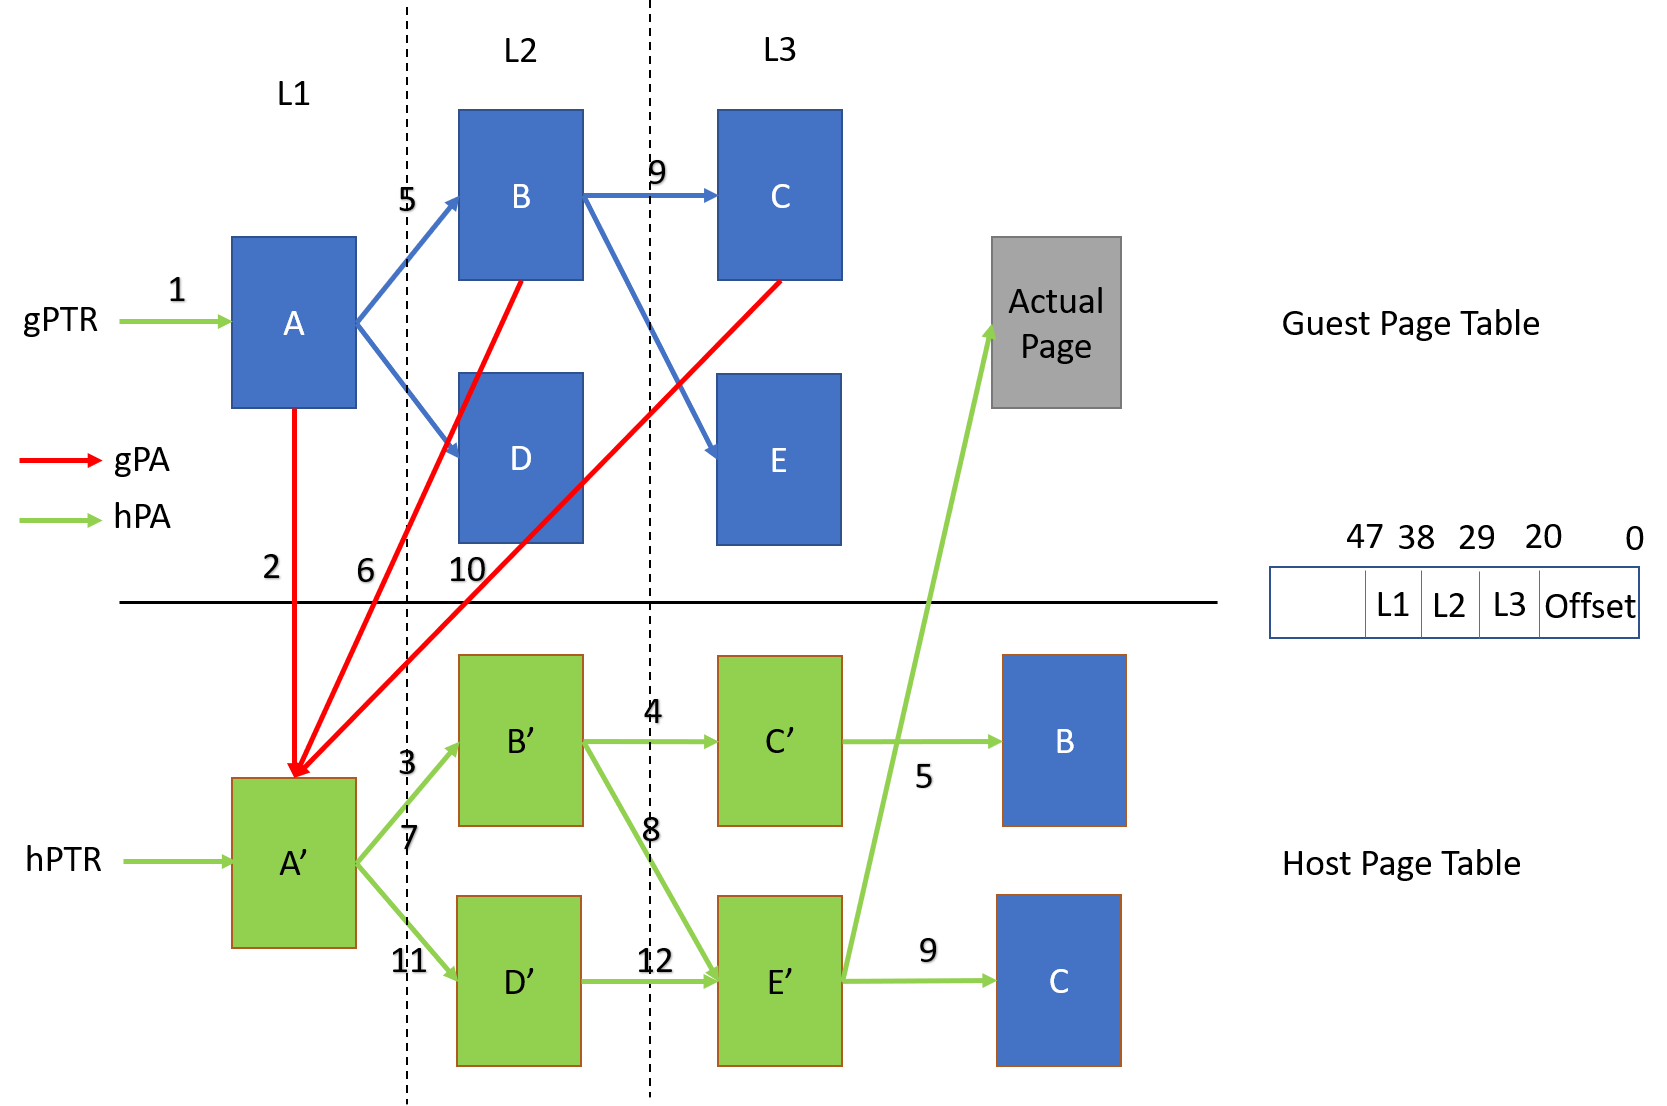
\includegraphics[scale=0.6]{1.png}
		\end{center}
	    The numbers on top of arrows indicate the sequence of page table walk. It requires 12 memory accesses to get the frame number of the desired physical page. Large page sizes help in reducing the latencies by increasing the TLB reach and reducing the no. of levels in a page table.
		
		\item The following workflow is taken from VMware workstation example consisting of a hosted system VM with three main components namely: VMApp (application portion of VMM), VMM (privileged monitor) and VMDriver (facilitates control transfer between host and VMM). 
		
	    \begin{center}
	    	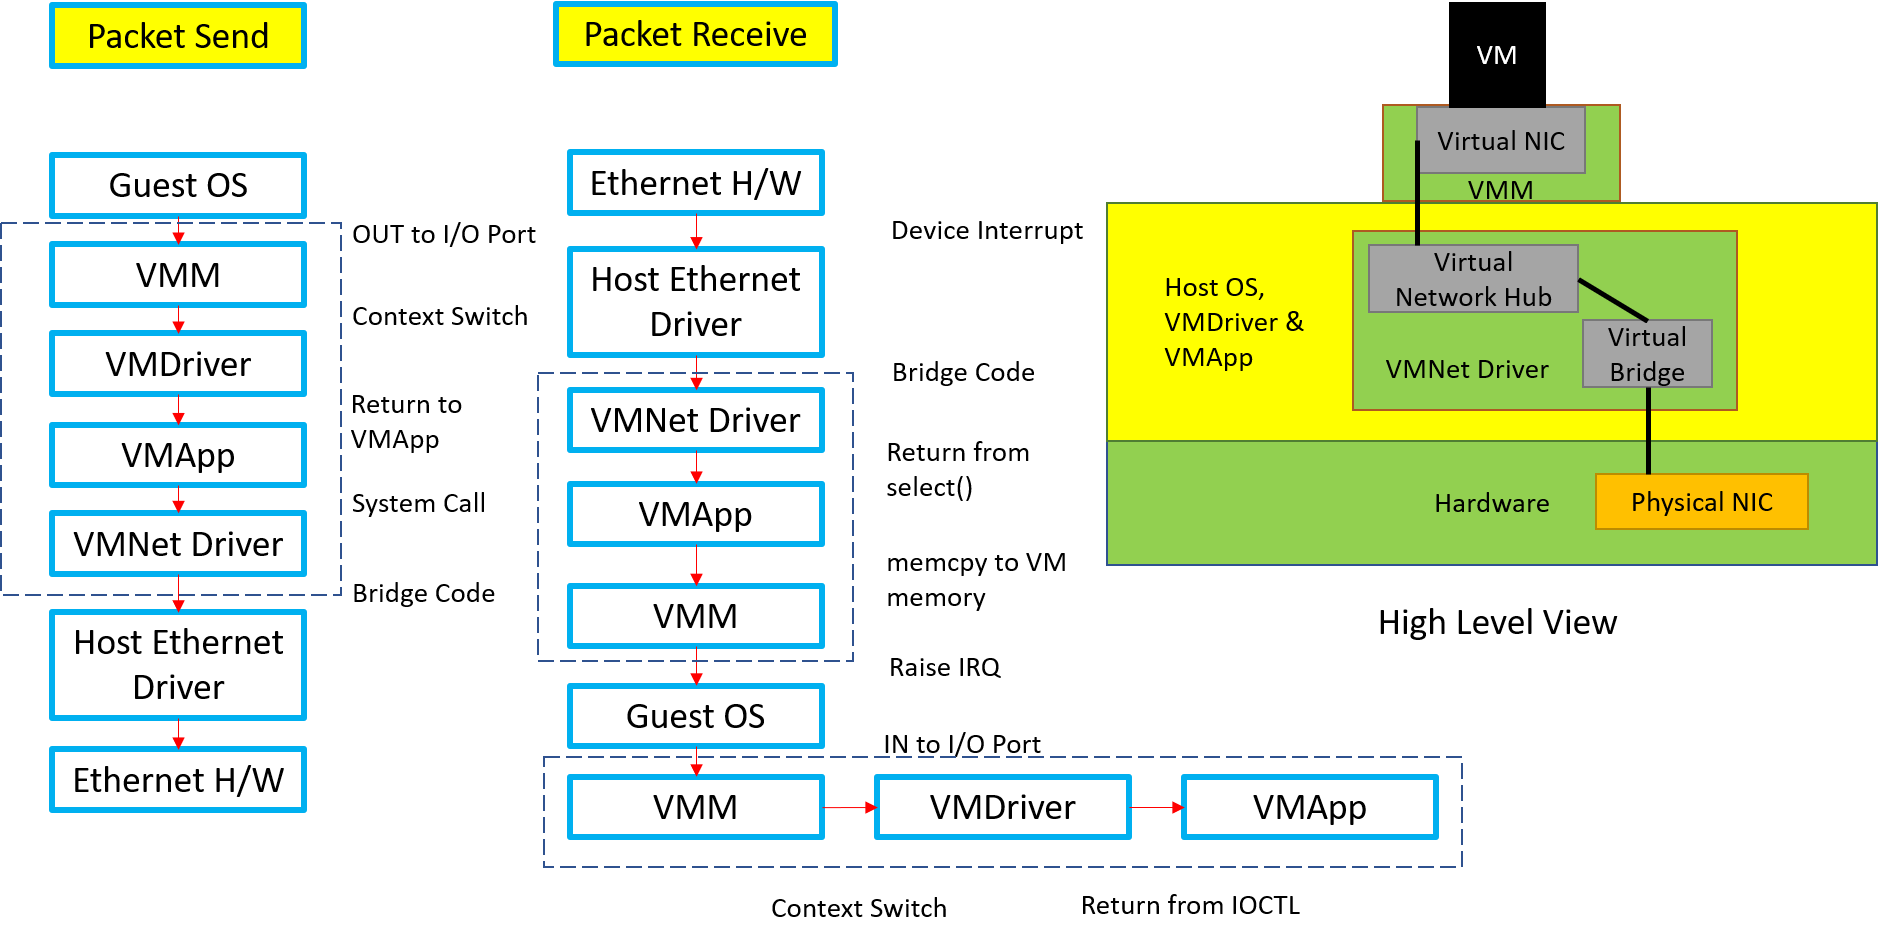
\includegraphics[scale=0.5]{2.png} \\
	    	Virtual NIC Workflow
	    \end{center}
    
       The following steps occur during a packet send operation,
       \begin{enumerate}
       	\item The guest OS driver initiates packet request by writing to virtual I/O ports which switches back to VMApp through the VMDriver
       	\item The VMApp makes a host OS system call which in turn invokes the VMNet driver
       	\item The VMNet driver runs the bridge code which forwards the packet to physical NIC through the host ethernet driver 
       \end{enumerate}
   
       The following steps occur during a packet receive operation,
       \begin{enumerate}
       	\item Packet receive happens in reverse. Bridged host NIC delivers the packet to VMNet. 
       	\item VMApp periodically runs select() to the VMNet and requests the VMM to raise a virtual IRQ if there is any incoming packet
       	\item The VMM posts the virtual IRQ and guest's driver issues a sequence of I.O accesses to ack. the receipt to the hardware
       \end{enumerate}
		
		
	        			
	\end{enumerate}
    
    \textbf{References}
    \begin{enumerate}
    	\item Jim Smith and Ravi Nair - Virtual Machines: Versatile Platforms for Systems and Processes 
    	\item Ludmila Cherkasova, Diwaker Gupta, and Amin Vahdat. 2007. Comparison of the three CPU schedulers in Xen. SIGMETRICS Perform. Eval. Rev. 35, 2 (September 2007), 42-51. DOI: https://doi.org/10.1145/1330555.1330556
    	\item https://docs.oracle.com/cd/E97728\_01/F12469/html/nestedpaging.html
    	\item https://docs.oracle.com/cd/E37670\_01/E37355/html/ol\_about\_hugepages.html
    	\item Jeremy Sugerman, Ganesh Venkitachalam, and Beng-Hong Lim. 2001. Virtualizing I/O Devices on VMware Workstation's Hosted Virtual Machine Monitor. In Proceedings of the General Track: 2001 USENIX Annual Technical Conference, Yoonho Park (Ed.). USENIX Association, Berkeley, CA, USA, 1-14
    	\item Course Lecture Notes   	
    \end{enumerate}
 

    
\end{document}